\chapter{results}\label{results}


\section{ghsep}\label{ghsep}

The random forest for the gamma-/hadron-separation gets trained on 
XXX diffuse gamma events and XXX diffuse proton events with a 5-fold cross-validation.
We define the class gamma to be of value 1 and protons of value 0.
The random forest thus predicts a "gammaness".
With these parameters, the distribution of the predicted "gammaness" 
is illustrated in figure \ref{fig:gh_sep}.

\begin{figure}
    \centering
    \includegraphics[page=2, width=.8\textwidth]{../analysis/plots/cross_val_sep_perf_plot.pdf}
    \caption{Distribution of the predicted gammaness on the cross-validated training data.
	    The two populations (Proton and Gamma, marked in blue and orange), can be separated 
	    to a certain degree. 
    A perfect prediction (AUC=1) would show no overlap between the distributions.}
    \label{fig:gh_sep}
\end{figure}

The ROC-curve is shown in figure \ref{fig:gh_roc}, with the model achieving an AUC of 
\num{0.835}.


\begin{figure}
    \centering
    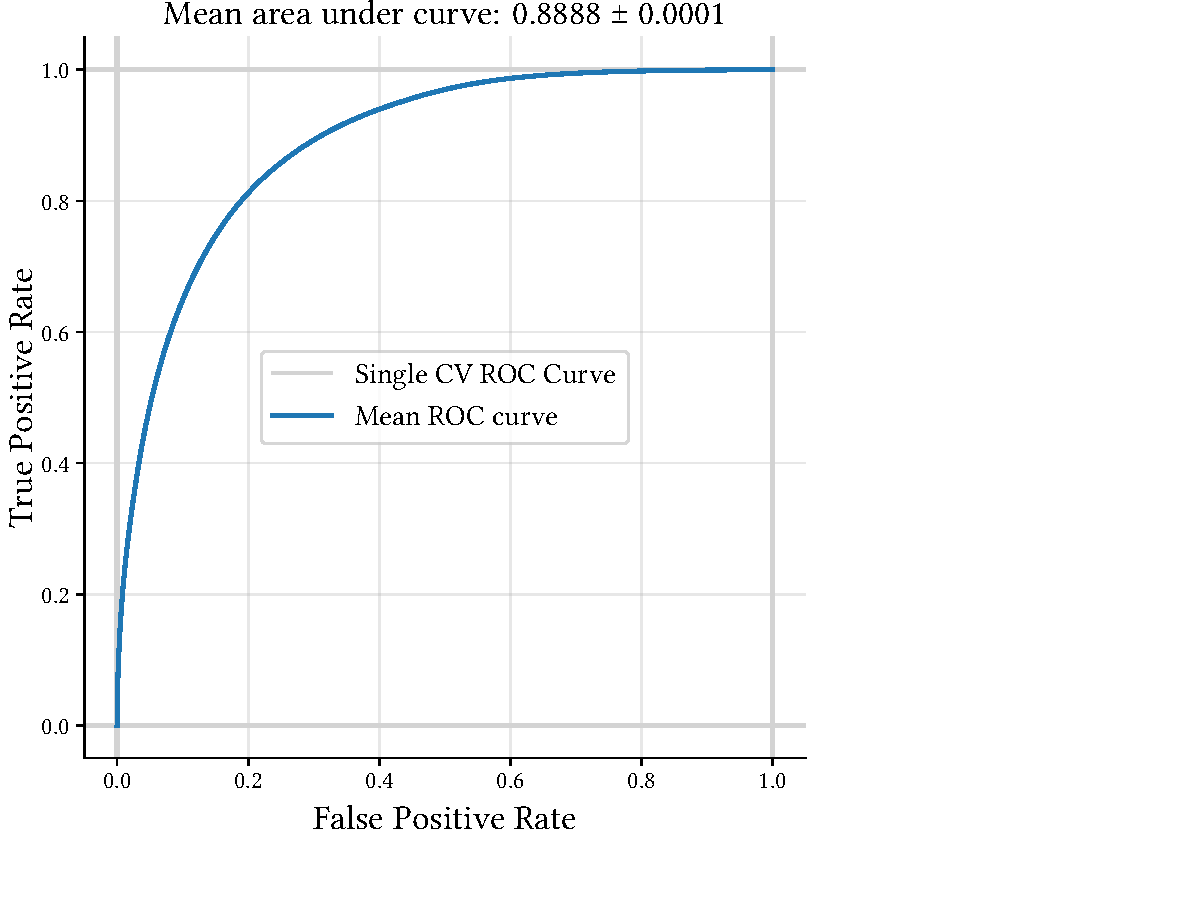
\includegraphics[page=1, width=.8\textwidth]{../analysis/plots/cross_val_sep_perf_plot.pdf}
    \caption{ROC-curve for the gamma/hadron separation on the cross validated training set 
    consisting of XXX proton events and YYY diffuse gamma events.
    The uncertainty "entspricht" the variance of the mean over the 5 cross-validation steps. 
    (make dummy column on the left to center properly?).}
    \label{fig:gh_roc}
\end{figure}


The feature importance, as calculated via sklearn, is shown in \ref{fig:gh_features}.
\begin{figure}
    \centering
    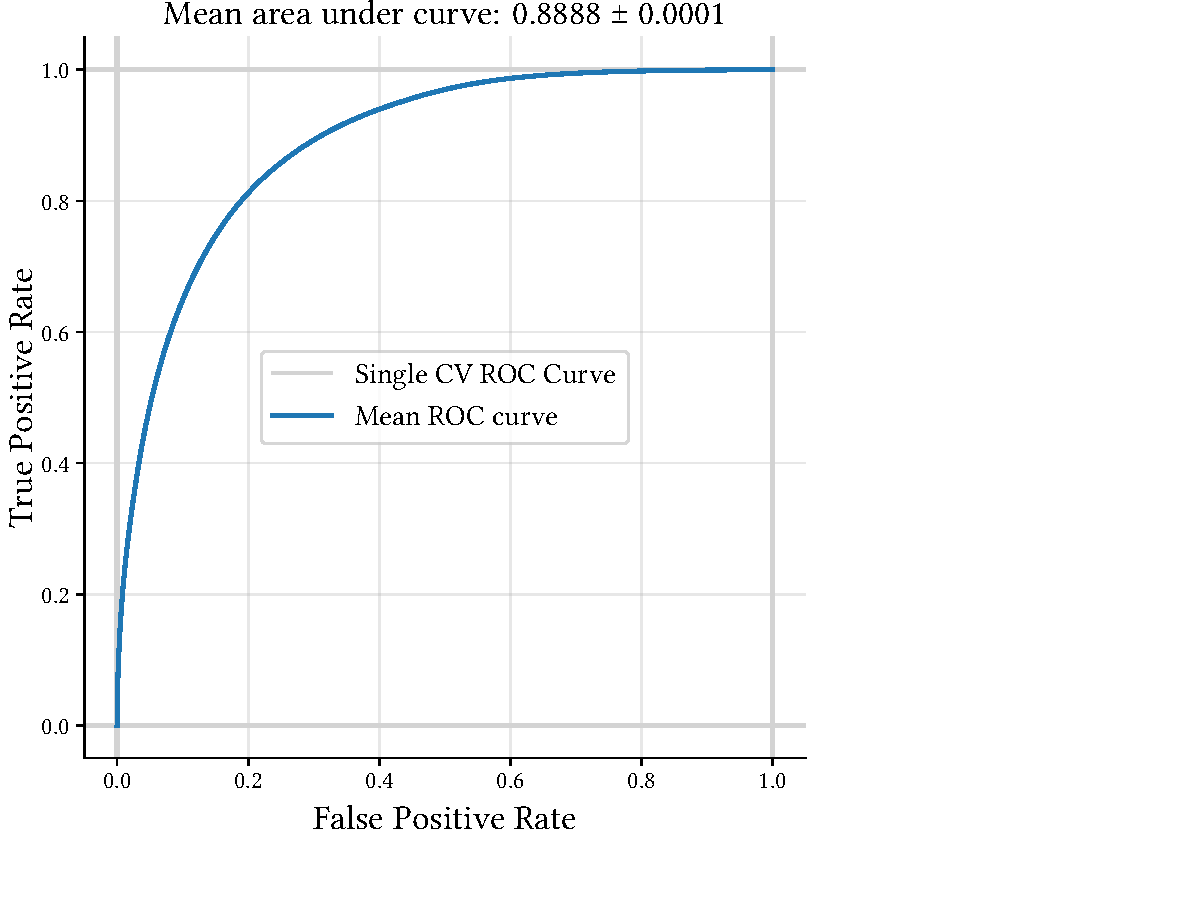
\includegraphics[page=1, width=.8\textwidth]{../analysis/plots/cross_val_sep_perf_plot.pdf}
    \caption{Feature importance for the gamma/hadron separation. Need to get that plot from the model!}
    \label{fig:gh_features}
\end{figure}


From our XXXX pointlike gamma events that we test our reconstruction method on, 
XXX \% get the correct label.
